\documentclass[a4paper,12pt]{article}
\usepackage[utf8]{inputenc}
\usepackage{amsmath, amssymb}
\usepackage{tikz}
\usetikzlibrary{trees}
\usepackage{algorithm}
\usepackage{algorithmic}

\title{3-adischer Steuerbaum mit Blockchain-Hash}
\author{Alexander Kern}
\date{\today}

\begin{document}
\maketitle

\section{Hierarchie des Baums}
Wir modellieren eine föderale Struktur als \textbf{3-adischen Baum}:
\begin{itemize}
    \item Ebene 0: Dörfer (1--3 pro Bezirk)
    \item Ebene 1: Bezirke (1--3 pro Bundesland)
    \item Ebene 2: Bundesländer (1--3 pro Land)
    \item Ebene 3: Länder (1--3 insgesamt)
\end{itemize}

\begin{center}
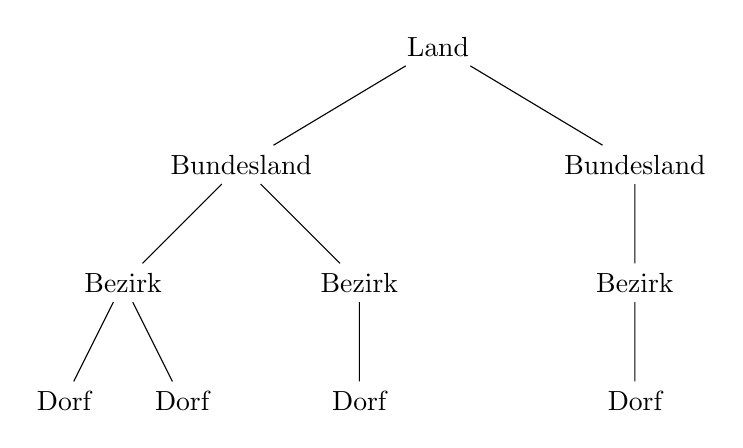
\begin{tikzpicture}[level distance=1.5cm,
  level 1/.style={sibling distance=5cm},
  level 2/.style={sibling distance=3cm},
  level 3/.style={sibling distance=1.5cm}]
\node {Land}
  child {node {Bundesland}
    child {node {Bezirk}
      child {node {Dorf}}
      child {node {Dorf}}
    }
    child {node {Bezirk}
      child {node {Dorf}}
    }
  }
  child {node {Bundesland}
    child {node {Bezirk}
      child {node {Dorf}}
    }
  };
\end{tikzpicture}
\end{center}

\section{Blockchain-Hash für jeden Knoten}
Jeder Knoten erhält einen Hash, der von seinem Namen, den Hashes seiner Kinder und dem Hash seines Elternknotens abhängt:

\begin{equation}
\text{hash}_\text{node} = H\Big(\text{name}_\text{node} \,\|\, \text{parent\_hash} \,\|\, \big\|_{c \in \text{children}} \text{hash}_c \Big)
\end{equation}

\section{Steueraggregation}
\subsection{Dorfebene}
Jedes Dorf erhebt eine lokale Steuer:

\begin{equation}
\text{tax}_\text{dorf} = \text{Einwohner} \times \text{Steuersatz}
\end{equation}

\subsection{Aggregation nach oben}
Die Steuer auf jeder Ebene ist die Summe der Steuern aller Kinder:

\begin{equation}
\text{tax}_\text{node} = \text{tax}_\text{local} + \sum_{c \in \text{children}} \text{tax}_c
\end{equation}

\subsection{Verteilung auf EU-Länder}
Am Ende kann die Steuer des Landes auf 1--3 EU-Länder verteilt werden:

\begin{equation}
\text{tax}_\text{EU\_Land} = \frac{\text{tax}_\text{Land}}{n_\text{EU-Länder}}, \quad 1 \le n_\text{EU-Länder} \le 3
\end{equation}

\section{Algorithmus: Baum erzeugen mit Hashes und Steuern}
\begin{algorithm}
\caption{Erzeuge 3-adischen Steuerbaum mit Blockchain-Hash}
\begin{algorithmic}[1]
\STATE \textbf{Input:} Ebenen: Land $\rightarrow$ Bundesland $\rightarrow$ Bezirk $\rightarrow$ Dorf
\STATE \textbf{Function} GenerateNode(level, depth, parentHash)
\STATE \quad Erzeuge Name für Knoten
\STATE \quad Falls Dorf: Steuer lokal zufällig setzen
\STATE \quad Falls depth > 0:
\STATE \quad \quad Wähle 1--3 Kinder
\STATE \quad \quad Rekursiv: GenerateNode(childLevel, depth-1, parentHash)
\STATE \quad Berechne node.hash = Hash(Name $\|$ parentHash $\|$ Kinderhashes)
\STATE \quad Berechne node.totalTax = tax\_local + Summe Kinder
\STATE \quad \textbf{return} node
\end{algorithmic}
\end{algorithm}

\section{Fazit}
Wir haben ein föderales Steuer-System modelliert, das:
\begin{itemize}
    \item 3-adisch aufgebaut ist
    \item Dörfer Steuern erheben, die nach oben aggregiert werden
    \item Blockchain-Hashes die Integrität sichern
    \item Am Ende die Steuern optional auf EU-Länder verteilen kann
\end{itemize}

\end{document}

